% !TEX root = ../masterthesis.tex
\chapter{Entangled photon generation using adiabatic rapid passage with frequency-chirped pulses}
\label{cha:chirp}

\section{Introduction and motivation}

In order to efficiently use the biexciton decay cascade, the \acl{XX} state has to be prepared beforehand in a robust way.
This chapter deals with the efficient inversion of the \ac{QD} from the ground state to the biexciton level via \ac{ARP}.
\acs{ARP} uses chirped pulses, which need to be measured and deterministically adjusted in order to effectively use them.
Therefore, the majority of this chapter will focus on the chirp and how to determine and adjust it, with the help of simulations and later with measurements.


\section{Chirp}
\label{sec:chirp}
A chirped signal is a signal whose frequency changes over time.
For example, the frequency of a linearly chirped signal $f(t)$ would be described by
\begin{equation}
f(t) = ct+f_0
\end{equation}
where $f_0$ is the starting frequency at $t=0$ and $c$ is the chirpyness. A linearly chirped sinusoidal wave is depicted in figure~\ref{fig:chirped-sin}.

\begin{figure}[H]
	\centering
	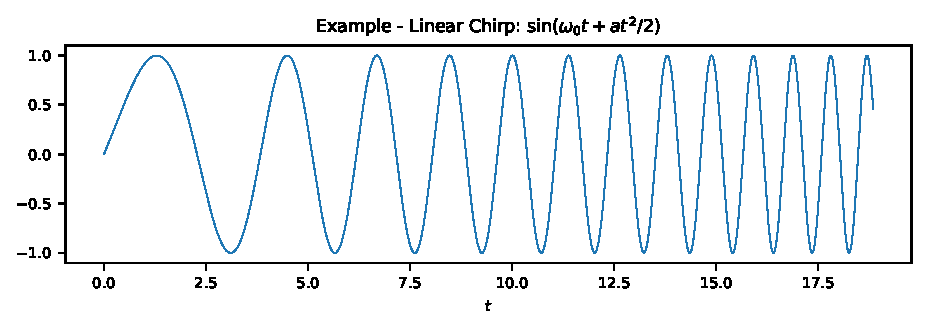
\includegraphics[width=\linewidth]{figures/chirp/plots/chirped-sin}
	\caption{A chirped sinusoidal wave which increases in frequency over time.}
	\label{fig:chirped-sin}
\end{figure}

As this chapter is concentrated on exciting \acp{QD} with frequency-chirped pulses, the mathematical description of chirped laser pulses will now be discussed. The shape of the electric field of a laser $E(t)$ can be approximated by
\begin{equation}
\label{eq:electric-field-laser}
E(t) \sim \mathrm{Re}\left(f^{1/2}(t) \cdot \exp\left(-i \omega t - i \phi(t)\right)\right)
\end{equation}
with the central frequency $\omega$ and the linear chirp $\phi(t)$.

Depending on the laser either a Gaussian or a hyperbolic secant describes the pulse shape more accurately~\cite{glassl_biexciton_2013, hirayama_real-time_2002}

\begin{itemize}
	\item Gaussian pulse:
	\begin{itemize}
		\item Pulse shape of
		\begin{equation}
		\label{eq:f_gauss}
		f_{gauss}(t) = \left(\frac{A_{gauss}}{\sqrt{2 \cdot \pi \cdot \tau_0 \cdot \tau}} \exp\left(-\frac{t^2}{2 \cdot \tau^2}\right)\right)^2
		\end{equation}
		with the normalization constant $A_{gauss}$, the pulse duration $\tau_0$, the central frequency $\omega$ and the chirp coefficient $\alpha$.
		\item Linear chirp of
		\begin{equation}
		\label{eq:phi-gauss}
		\phi_{gauss}(t) = \frac{a_{gauss} t^2}{2}
		\end{equation}
		where 
		\begin{equation}
		\tau = \sqrt{\alpha^2 / \tau_0^2 + \tau_0^2}
		\end{equation}
		characterizes the chirped pulse length and
		\begin{equation}
		\label{eq:chirp-parameter}
		a = \alpha / (\alpha ^ 2 + \tau _0 ^ 4)
		\end{equation}
		is the frequency chirp rate.
	\end{itemize}
	\newpage
	\item Secant pulse:
	\begin{itemize}
		\item Pulse shape of
		\begin{equation}
		f_{secant}(t) = A_{secant} \cdot \textrm{sech}^2\left(\frac{t}{\tau_0}\right) = A_{secant} \cdot \left(\frac{2}{\exp(\frac{t}{\tau_0}) + \exp(-\frac{t}{\tau_0})}\right)^2
		\end{equation}
		with the normalization constant $A_{secant}$, the pulse duration $\tau_0$, the central frequency $\omega$ and the chirp coefficient $\alpha$.
		\item Linear chirp of
		\begin{equation}
		\phi_{secant}(t) = \alpha_{secant}\left(\frac{t}{\tau_0}\right)^2
		\end{equation}
	\end{itemize}
\end{itemize}

The following discussion will assume a Gaussian laser shape as described by equation~\eqref{eq:f_gauss} and \eqref{eq:phi-gauss}.
A simulation for $E$ is plotted in figure~\ref{fig:chirpedlaserpulse} for different chirp parameters $\alpha$ suitable to display examples for strong and weak chirps.
As can be seen there, the chirp parameter strongly influences the shape of the electric field.
If $E$ could be measured directly, the chirp could be easily estimated.
This is not feasible in our case, as our Ti:Sa laser can produce laser pulses as short as \SI{100}{\femto \second} and response times of photodiodes and oscilloscopes are in the best case in the order of \SI{200}{\femto \second}.
This means they cannot even measure the duration of these ultrashort pulses let alone resolve the pulse shape.

\begin{figure}[H]
	\centering
	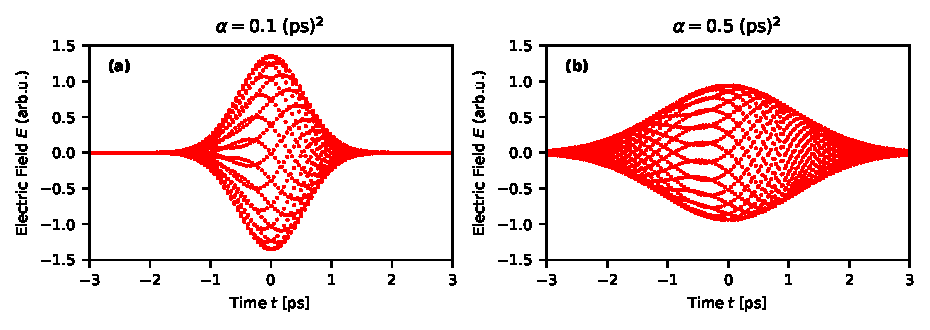
\includegraphics[width=\linewidth]{figures/chirp/plots/chirped_laser_pulse}
	\caption{Electric field $E$ of Gaussian laser pulse of pulse duration $\tau_0=\SI{0.5}{\pico \second}$ for chirp of (a) $\alpha = \SI{0.1}{\pico \second \squared}$ and (b) $\alpha = \SI{0.5}{\pico \second \squared}$}
	\label{fig:chirpedlaserpulse}
\end{figure}

\newpage

\section{Measuring the chirp with interferometric autocorrelation}
\begin{figure}[H]
	\centering
	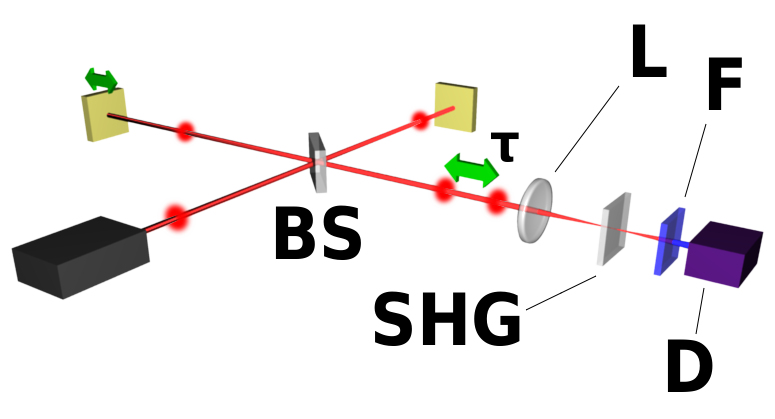
\includegraphics[width=0.6\linewidth]{figures/chirp/Optical-interferometric-autocorrelation-setup.png}
	\caption[Schematics of an interferometric autocorrelator]{Schematics of an interferometric autocorrelator, where \textbf{L} is a converging lens, \textbf{SHG} a second-harmonic generation crystal, \textbf{BS} a beam splitter, \bm{$\tau$} the interval between two pulses, \textbf{D} the detector and \textbf{F} a spectral filter to block the fundamental wavelength~\cite{noauthor_optical_nodate}.}
	\label{fig:optical-field-autocorrelation-setup}
\end{figure}
In order to estimate the pulse width $\tau_0$, \ac{IAC} is used.
Basically, a nonlinear crystal is added to a Michelson interferometer in order to generate a signal governed by
\begin{equation}
\label{eq:i-m-integral}
I_M(\tau) = \int_{-\infty}^{+\infty}\langle|(E(t)+E(t-\tau))^2|^2\rangle dt.
\end{equation}
and plotted in figure~\ref{fig:imgausschirpwithoutslitwithoutmosaic}~\cite{diels_ultrashort_2006}.
Here, $\langle \rangle$ denotes averaging over fast oscillations of the electric field.
\begin{figure}[H]
	\centering
	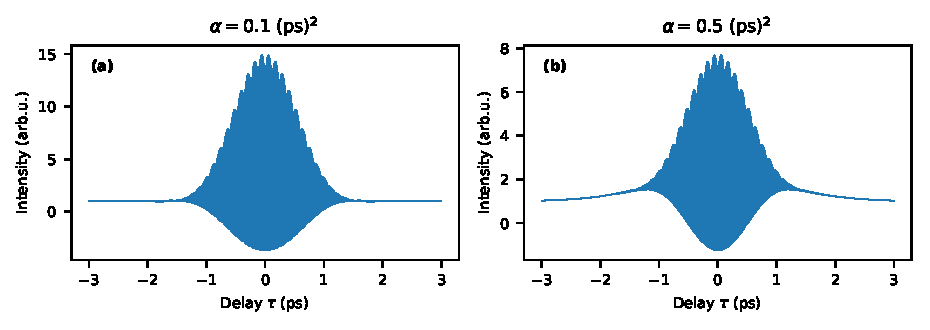
\includegraphics[width=\linewidth]{figures/chirp/plots/I_M_gauss_chirp_without_slit_without_MOSAIC}
	\caption{Intensity of IAC of a Gaussian laser pulse of pulse duration $\tau_0=\SI{0.5}{\pico \second}$ without applied MOSAIC filter for chirp of (a) $\alpha = \SI{0.1}{\pico \second \squared}$ and (b) $\alpha = \SI{0.5}{\pico \second \squared}$}
	\label{fig:imgausschirpwithoutslitwithoutmosaic}
\end{figure}
Under the use of equation~\ref{eq:electric-field-laser}, equation~\eqref{eq:i-m-integral} can be expanded to
\begin{align}
I(\tau) = 1 &+ 2 \int f(t) f(t + \tau) dt + \int f(t) f(t + \tau) \cos(2 \omega \tau + 2 \Delta \phi) dt \nonumber\\
&+ 2 \int f^{1/2}(t) f^{3/2}(t + \tau) \cos(\omega \tau + \Delta \phi) dt + 2 \int f^{3/2}(t) f^{2/2}(t + \tau) \cos(\omega \tau + \Delta \phi) dt
\end{align}
where $\Delta \phi(t, \tau) = \phi(t + \tau) - \phi(t)$ and $\int f(t) dt = 1$.

As can be seen in figure~\ref{fig:imgausschirpwithoutslitwithoutmosaic}, the chirp parameter $\alpha$ has hardly any measurable influence on the resulting signal.
However, certain modifications to the \ac{IAC} signal introduced by \textcite{hirayama_real-time_2002} make it much more sensitive to the temporal chirp.
It is called \ac{MOSAIC} and performs the following transformations on the \ac{IAC} spectrum: The $\omega$ terms are eliminated and the $2\omega$ term is doubled.
The \ac{MOSAIC} signal is then described by
\begin{equation}
\label{eq:i-m-filtered}
I_{M}(\tau) = 1 + 2 \int f(t) f(t + \tau) dt + 2 \int f(t) f(t + \tau) \cos(2\omega \tau + 2\Delta \phi) dt.
\end{equation}
When the MOSAIC filter is applied to the data in figure~\ref{fig:imgausschirpwithoutslitwithoutmosaic}, this results in a signal as shown in figure~\ref{fig:mosaicchirpedlaserpulse}.
Here the influence of the chirp is clearly visible in the lower envelope.
\begin{figure}[H]
	\centering
	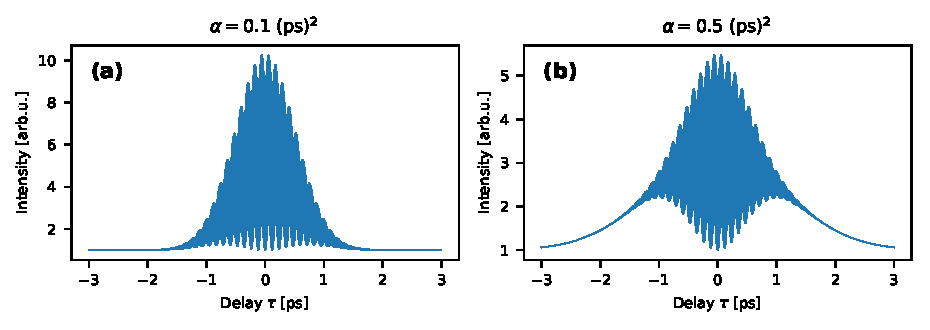
\includegraphics[width=\linewidth]{figures/chirp/plots/mosaic_chirped_laser_pulse}
	\caption{Intensity of IAC of a Gaussian laser pulse of pulse duration $\tau_0=\SI{0.5}{\pico \second}$ for chirp of (a) $\alpha = \SI{0.1}{\pico \second \squared}$ and (b) $\alpha = \SI{0.5}{\pico \second \squared}$}
	\label{fig:mosaicchirpedlaserpulse}
\end{figure}

\newpage

The points of the lower envelope can be obtained by determining the local minima of the signal as shown in figure~\ref{fig:mosaicchirpedlaserpulsefindenvelope}.

\begin{figure}[H]
	\centering
	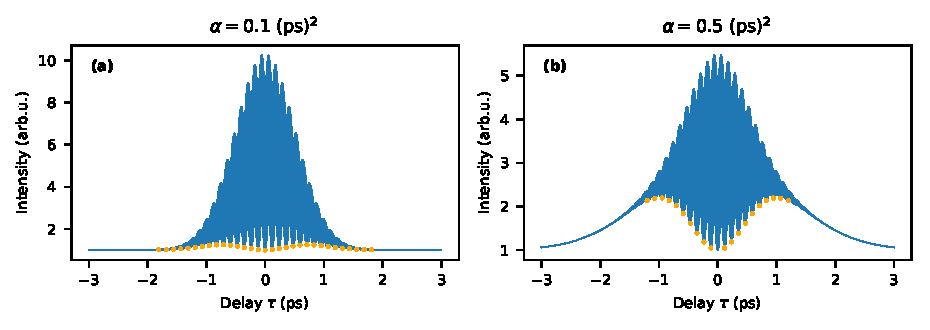
\includegraphics[width=\linewidth]{figures/chirp/plots/mosaic_chirped_laser_pulse_find_envelope}
	\caption{Intensity of IAC of a Gaussian laser pulse of pulse duration $\tau_0=\SI{0.5}{\pico \second}$ with applied MOSAIC filter for chirp of (a) $\alpha = \SI{0.1}{\pico \second \squared}$ and (b) $\alpha = \SI{0.5}{\pico \second \squared}$.
		The orange dots are results of a numerical peak finder algorithm, executed in order to find local minima.}
	\label{fig:mosaicchirpedlaserpulsefindenvelope}
\end{figure}

The lower bound (minima envelope) of the MOSAIC trace can be derived by use of a standard textbook procedure~\cite{klein_optics_1986}
\begin{equation}
S^{min}_{MOSAIC}(\tau)= 1 + 2 \cdot g(\tau) - 2 \cdot [g_s^2(\tau)+g_c^2(\tau)]^{1/2}
\end{equation}
with
\begin{align}
g(\tau)&=\int f(t)f(t+\tau)dt\\
g_s(\tau)&=\int f(t)f(t+\tau)sin(2\Delta\phi)dt\\
g_c(\tau)&=\int f(t)f(t+\tau)cos(2\Delta\phi)dt.
\end{align}
The points of the lower envelope determined before can now be fitted in order to obtain the chirp parameter $\alpha$ as shown in figure~\ref{fig:mosaicchirpedlaserpulsefitenvelope}.
It is visible that the fitted values of $\alpha$ correspond to the expected values.
\begin{figure}[H]
	\centering
	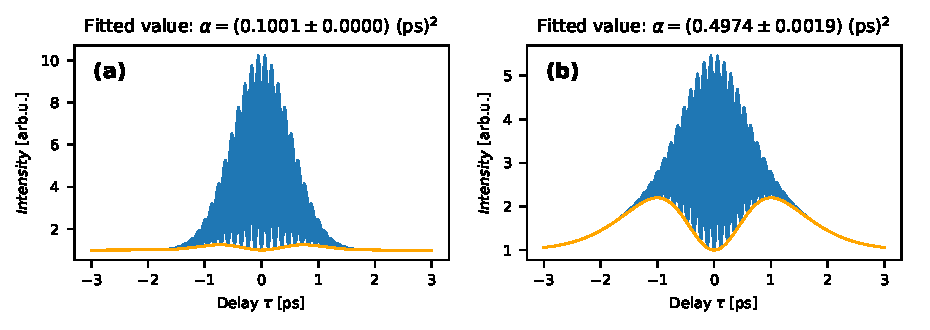
\includegraphics[width=\linewidth]{figures/chirp/plots/mosaic_chirped_laser_pulse_fit_envelope}
	\caption[Intensity of IAC of a Gaussian laser pulse of pulse duration $\tau_0=\SI{0.5}{\pico \second}$ with applied MOSAIC filter and fitted $\alpha$-values.]{Intensity of IAC of a Gaussian laser pulse of pulse duration $\tau_0=\SI{0.5}{\pico \second}$ with applied MOSAIC filter for chirp of (a) $\alpha = \SI{0.1}{\pico \second \squared}$ and (b) $\alpha = \SI{0.5}{\pico \second \squared}$.
		The orange line is a fit for the lower envelope of the MOSAIC signal in order to obtain~$\alpha$.}
	\label{fig:mosaicchirpedlaserpulsefitenvelope}
\end{figure}

\section{Deterministically adjusting the chirp with a pulse expander}
\label{sec:pulse-expander}
\begin{figure}[H]
	\centering
	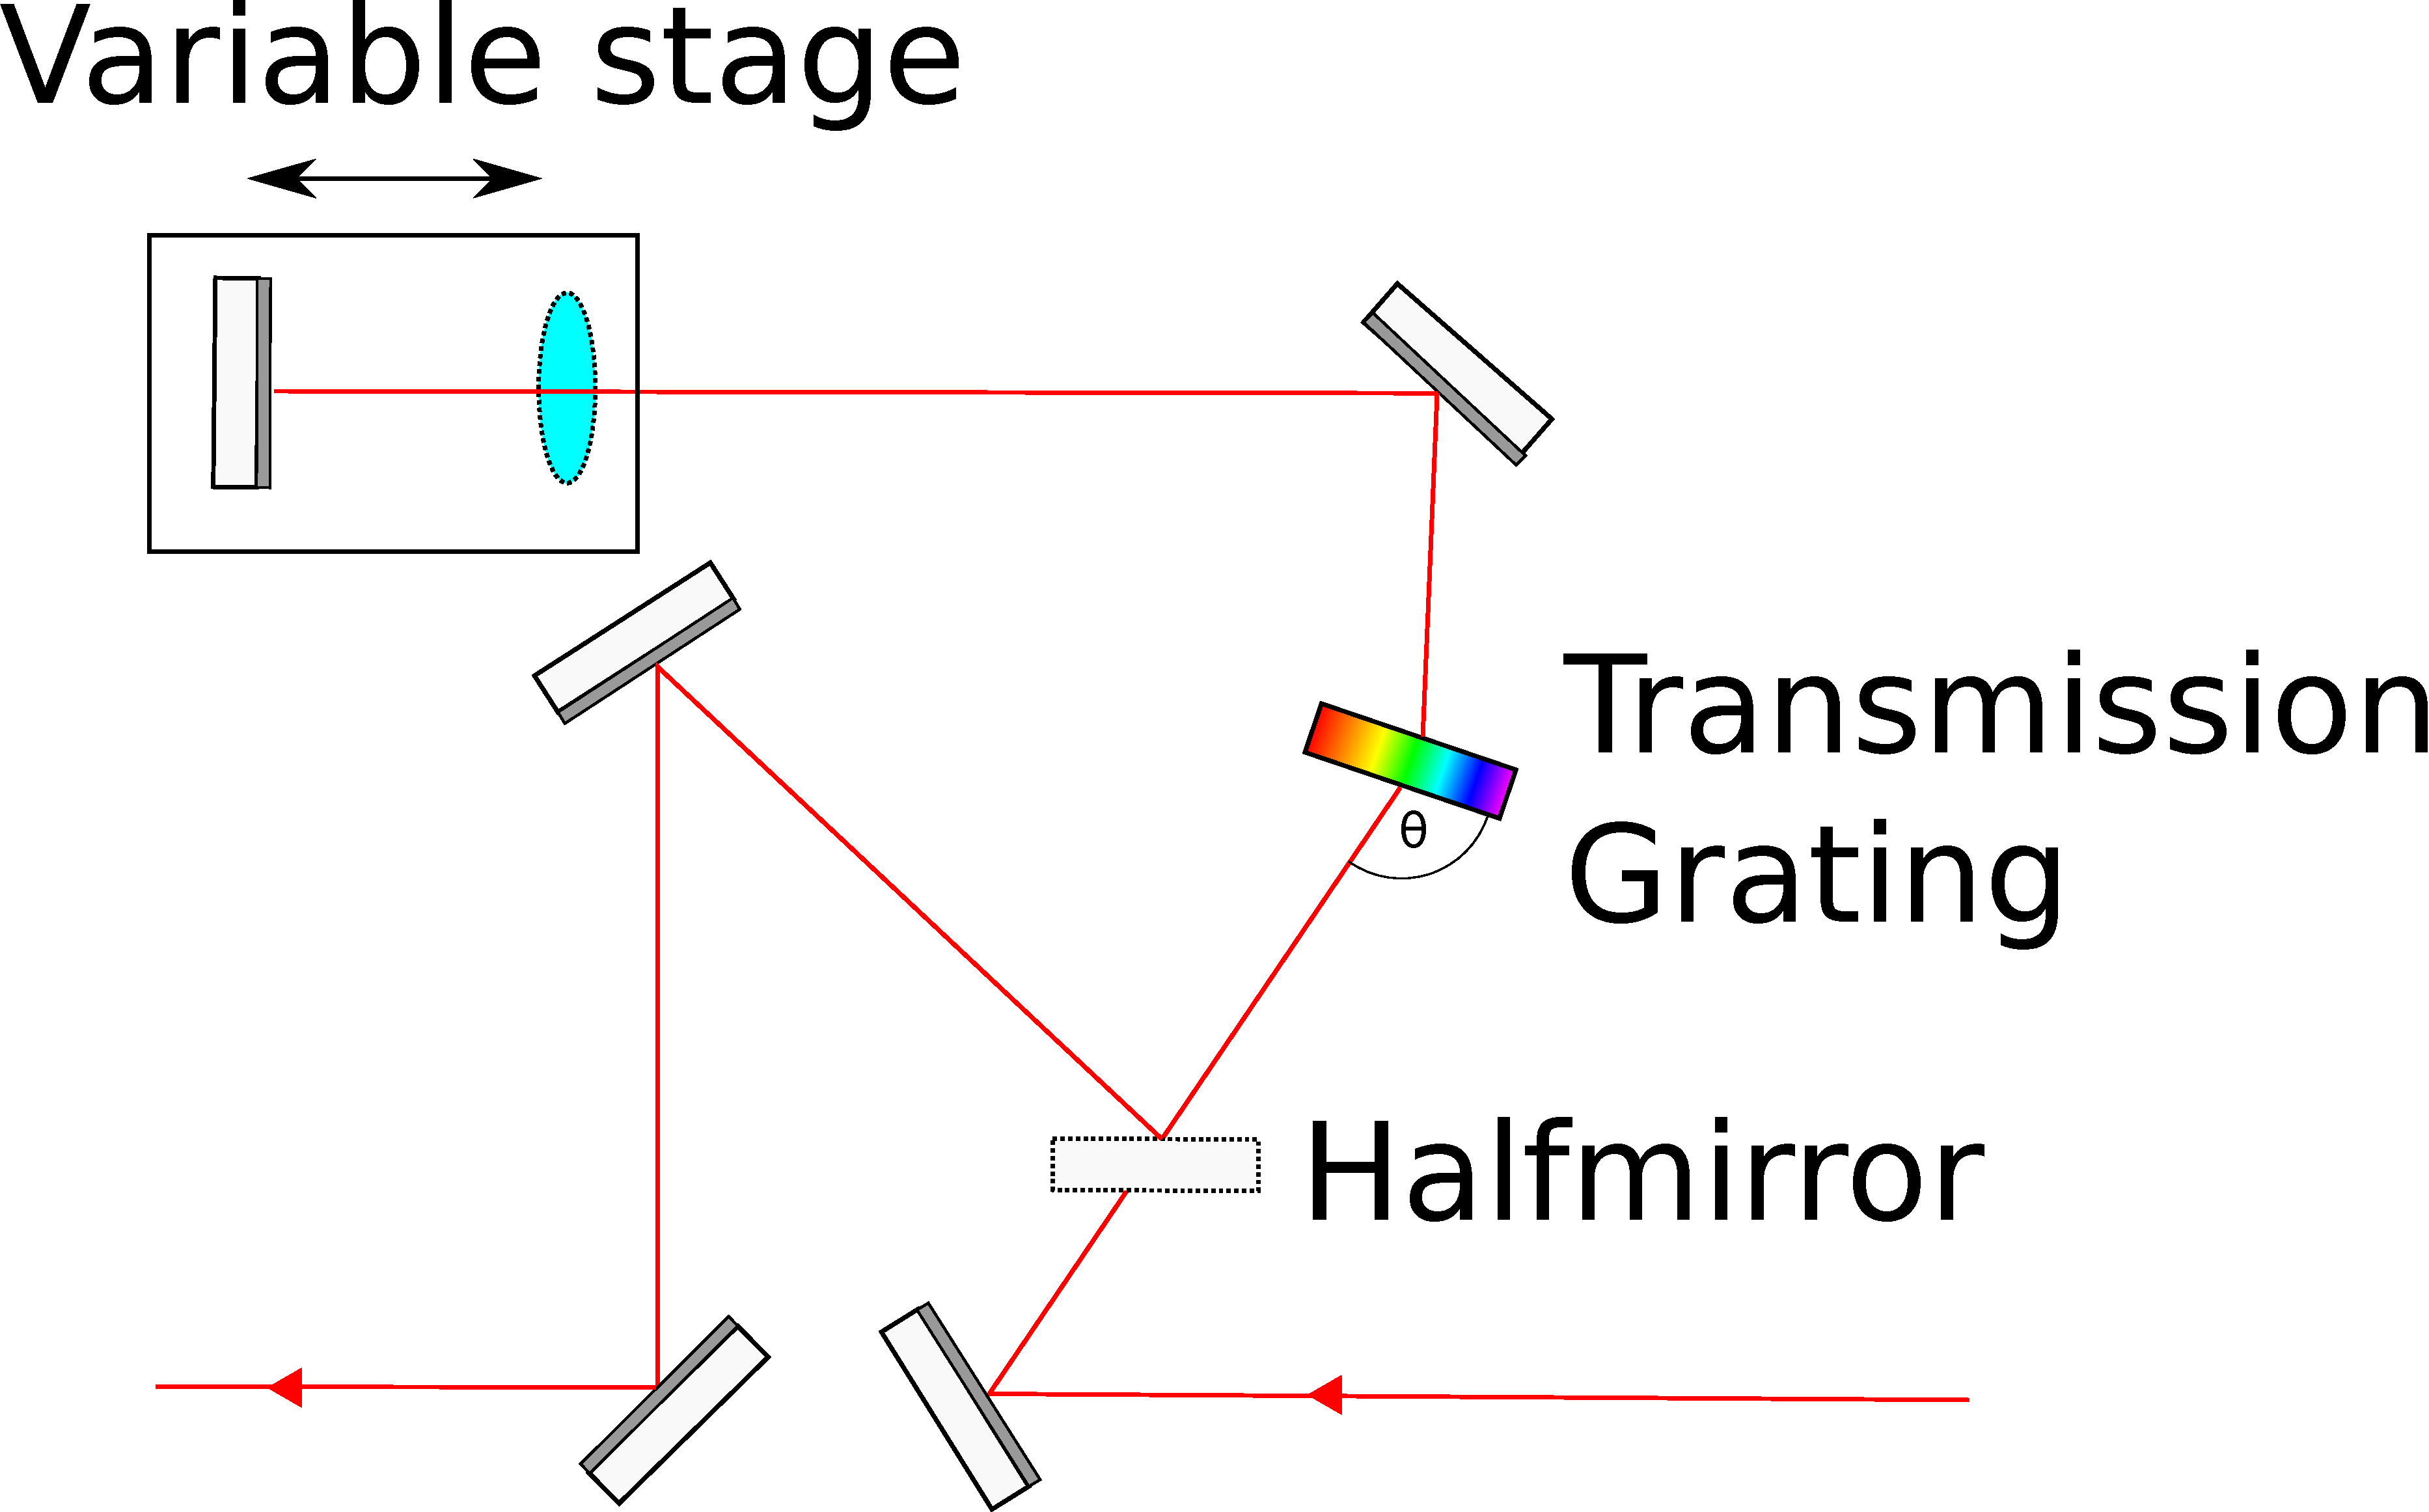
\includegraphics[width=0.7\linewidth]{figures/chirp/pulse-expander}
	\caption{Scheme of a folded pulse expander as described by \textcite{martinez_3000_1987}.
		The light enters on the right side, passes the halfmirror, and enters the system of transmission grating, lens and mirrors.
		Afterwards it hits the halfmirror and exits on the left hand.
		It induces an accumulated group velocity dispersion on the signal depending on the optical distance between the transmission grating and the lens.}
	\label{fig:pulse-expander}
\end{figure}



In the optimal case the chirp of the pulse can be deterministically adjusted in order to most efficiently excite the \ac{QD} via adiabatic rapid passage (going to be introduced in section~\ref{sec:arp}).
Grating compressors as discussed by \textcite{martinez_3000_1987} were originally used to compensate the broadening effect fibers have on pulses.
However, together with a telescope they have the inverse effect and can be used to induce a chirp.
A setup like this is sketched in figure~\ref{fig:pulse-expander} and it will in future references in this work be called \textit{pulse expander}.
Its main elements are a transmission grating and a lens.
This folded setup uses a mirror after the lens in order to need only one lens and mirror.
The accumulated group velocity dispersion $\frac{d^2 \Phi}{d \omega^2}$ can be adjusted by varying the optical distance $d$ between the focal plane of the lens and the transmission grating and is described by
\begin{equation}
\frac{d^2 \Phi}{d \omega^2} = k \beta^2 2 d
\end{equation}
where $k$ is the wavenumber and $\beta$ is given by
\begin{equation}
\beta = \frac{\lambda}{2 \pi \omega_0 \cos \theta}
\end{equation}
with $\lambda$ denoting the centre wavelength, $w_0$ the beam waist (beam size at the point of its focus) and $\theta$ the emerging angle as sketched in figure~\ref{fig:pulse-expander}.

\begin{figure}[H]
	\centering
	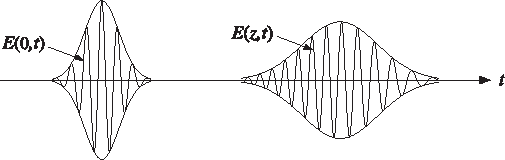
\includegraphics[width=0.7\linewidth]{figures/chirp/group-velocity-dispersion}
	\caption{Influence of group velocity dispersion for example inside a fiber on a Gaussian pulse~\cite{orfanidis_electromagnetic_2002}}
	\label{fig:group-velocity-dispersion}
\end{figure}

As can be seen in figure~\ref{fig:group-velocity-dispersion}, a group velocity dispersion has a similar effect on a Gaussian pulse as a chirp.
In fact, the frequency chirp rate $a_{gauss}$ introduced in equation~\eqref{eq:phi-gauss} can be put into relation with it by:~\cite{orfanidis_electromagnetic_2002}
\begin{equation}
a_{gauss} = \frac{\frac{d^2 \Phi}{d \omega^2}}{\tau_0^4 + \left(\frac{d^2 \Phi}{d \omega^2}\right)^2}
\end{equation}



\section{Adiabatic rapid passage}
\label{sec:arp}
One way to invert the \ac{QD} from the ground state $\ket{G}$ to the biexciton state $\ket{XX}$ is by exciting it with a narrow-band laser pulse of constant centre frequency, which equals to half of the ground state biexciton transition frequency.
As described in equation~\eqref{eq:n-xx}, if the pulse area $\theta=\pi$, a population inversion from the $\ket{G}$ state to the $\ket{XX}$ occurs.
However, the $\pi$-pulse method is not a generally robust scheme.
In order to ensure the inversion, precise control of the field intensity is required~\cite{glassl_biexciton_2013}.
Adiabatic rapid passage \acused{ARP} (\acs{ARP}) with frequency chirped pulses is a much more robust alternative to this Rabi-flopping scheme.
Here, the frequency of the laser signal is swept through resonance, starting slightly above or below the resonance frequency.
The biexciton state can be populated with nearly perfect efficiency~\cite{glassl_biexciton_2013} if the process is performed adiabatically, i.e. if~\cite{malinovsky_general_2001}
\begin{equation}
\Omega_0^2 \gg |\frac{d}{dt} \omega(t)|
\end{equation}
where $\Omega_0$ is the peak Rabi frequency and $\omega(t)$ is the center frequency of the laser pulse. 

In figure~\ref{fig:biexciton-occupation} simulations in order to determine the final biexciton occupation for different biexciton binding energies $\Delta$ by \textcite{glassl_biexciton_2013} are presented.
Here, a linearly-chirped Gaussian laser pulse as discussed in section~\ref{sec:chirp} was assumed.
\begin{figure}[H]
	\centering
	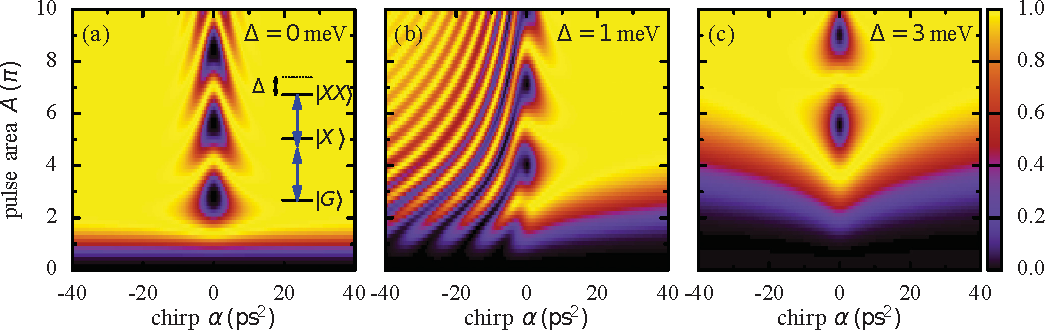
\includegraphics[width=\linewidth]{figures/chirp/biexciton-occupation}
	\caption[Final biexciton occupation after chirped Gaussian pulse of pulse duration $\tau_0 = \SI{2}{\pico \second}$]{Final biexciton occupation after chirped Gaussian pulse of pulse duration $\tau_0 = \SI{2}{\pico \second}$.
		It is plotted against the original pulse area $A$ (vertical axis) and the chirp parameter $\alpha$ for biexciton binding energies of (a) $\Delta=0$, (b) 1, and (c) \SI{3}{\milli \electronvolt}~\cite{glassl_biexciton_2013}.}
	\label{fig:biexciton-occupation}
\end{figure}
The central frequency is chosen so that for $\alpha=0$ it resonates to groundstate-to-biexction transition, which is sketched in figure~\ref{fig:biexciton-occupation}.
For $\alpha=0$ Rabi oscillations are visible and their period depends strongly on the biexciton binding energy $\Delta$.
However, for $\alpha \gg 0$ biexciton preparation becomes insensitive to small variations of the pulse area $A$ as long it exceeds a certain threshold.
This is therefore the regime which would be the most suitable to work in.
In the case of $\alpha < 0$ this insensitivity does not appear for moderate values of $\Delta$ as can be seen in figure~\ref{fig:biexciton-occupation}(b).

\newpage
\section{Measurements and discussion}
As discussed in the sections above, the final goal is to excite a \ac{QD} via \ac{ARP}.
The first step to do that is to determine the chirp of a laser pulse which only passed the pulse shaper with the \ac{IAC}.
Here a laser pulse of only $\tau_0=\SI{344}{\femto \second}$ was used as the \ac{IAC} can not resolve fine enough details for greater $\tau_0$.
Even though broader peaks will be necessary in order to excite the \ac{QD} with \ac{ARP}, this is not a problem as the equivalent chirp can be calculated for greater $\tau_0$ with equation~\eqref{eq:chirp-parameter}.

Afterwards, a signal was measured after passing a pulse expander as discussed in section~\ref{sec:pulse-expander} and sketched in figure~\ref{fig:setupflat}.
The comparison between these two is shown in figure~\ref{fig:measuredchirpedlaserpulsebeforemosaic}.
Compared to the simulations in figure~\ref{fig:imgausschirpwithoutslitwithoutmosaic} it is visible that the \ac{IAC} of the laser pulse without the pulse expander fits the expected shape well, while the one with the pulse expander does not.
Possible reasons could be that the chirp is too high for the model used in the simulation to work or that the pulse expander introduces side effects not considered in the simulation.

\begin{figure}[H]
	\centering
	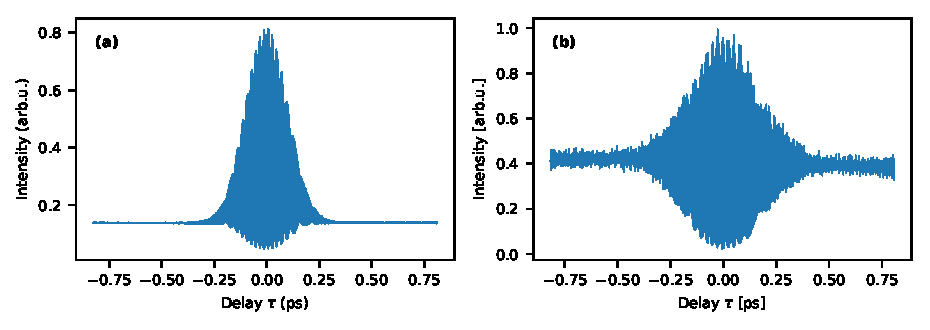
\includegraphics[width=\linewidth]{figures/chirp/plots/measured_chirped_laser_pulse_before_MOSAIC}
	\caption{Measured IAC of Ti:Sa Laser without (a) and with (b) pulse expander before the autocorrelator.}
	\label{fig:measuredchirpedlaserpulsebeforemosaic}
\end{figure}

The same signals after applying the \ac{MOSAIC} filter are shown in figure~\ref{fig:measuredchirpedlaserpulseaftermosaic}.
It is visible that the lower envelopes in figure~\ref{fig:measuredchirpedlaserpulseaftermosaic}(a) and \ref{fig:measuredchirpedlaserpulseaftermosaic}(b) do not resemble the expected ones in figure~\ref{fig:mosaicchirpedlaserpulse}.
As the laser signal without pulse expander was assumed to be relatively unchirped, it is already unexpected that the lower envelope differs that much from a constant line at zero intensity.
One explanatory approach could be that the laser was already chirped to begin with. However, this would not explain why the shape of the lower envelope differs from the characteristic one of the simulation.
The next approach was to send the laser without pulse shaper into the \ac{IAC}.
However, the envelope of the signal after applying the \ac{MOSAIC} filter showed no visible difference to the signal which has not passed a pulse shaper (depicted in figure~\ref{fig:measuredchirpedlaserpulseaftermosaic}).

\begin{figure}[H]
	\centering
	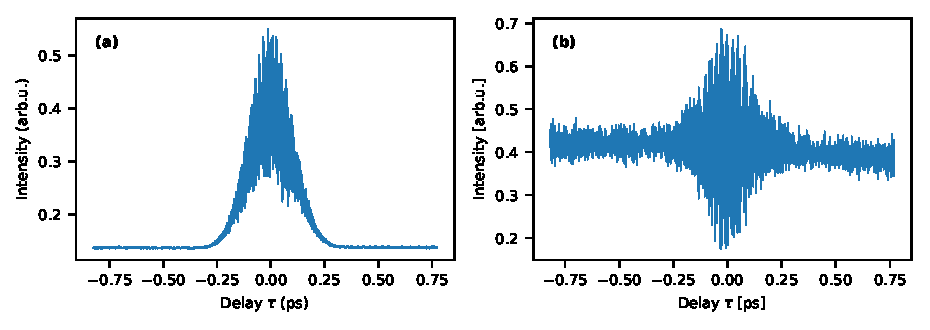
\includegraphics[width=\linewidth]{figures/chirp/plots/measured_chirped_laser_pulse_after_MOSAIC}
	\caption{Measured IAC of Ti:Sa Laser with applied MOSAIC filter without (a) and with (b) pulse expander before the autocorrelator.}
	\label{fig:measuredchirpedlaserpulseaftermosaic}
\end{figure}

The next step would have been to deterministically excite the \ac{QD} with \ac{ARP}.
However, it might be advisable to repeat the same procedure with another ultrashort pulsed laser before in order to rule out that our laser is already heavily chirped to begin with.
Alternatively, \ac{ARP} with the pulse expander can be attempted without measuring the chirp first and iteratively adjusting the lens-grating distance until the optimum is reached. 